\documentclass{ximera}
% \handouttrue
%%% Where to find images
\graphicspath{  %% When looking for images,
{./}            %% look first at your level,
{./basics/}     %% then in this folder,
}    
%\addPrintStyle{..}

\author{Wim Obbels \and Bart Snapp}
\title{First Topic}

\begin{document}
\begin{abstract}
    A simple module written in Ximera.
\end{abstract}
\maketitle
\label{xim:ximeraDemo}

This is an example of a Ximera activity that may contain discussion as well as
questions. We give examples
with some useful \hyperref[xim:ximeraEnvironments]{environments} and
\hyperref[xim:ximeraCommands]{commands}.

The first thing to note is that the title of the document is the same as the
title of the source file, and this is the same as the title of the folder
containing this files.
This is \textbf{not necessary}; however adhearing to a standard like this will
make your work easier to debug and share with others for years to come.

% Demo: small adhoc differences between PDF and HTML version
\pdfOnly{
    \begin{remark}
        It is advisable to also view the Online version, where this remark
        refers to the PDF.
        \ifhandout
            By the way, you are using the \textit{handout} PDF, which does
            \textbf{not} contain answers. \\
            There is also a so-called \textit{standard} PDF \textit{which does
                contain answers and hints}.
        \else
            You are, by the way, using the so-called \textit{standard} PDF,
            which \textbf{contains the answers} to the exercises. \\
            There is also a \textit{handout} PDF \textit{without the answers}.
        \fi
    \end{remark}
}
\begin{onlineOnly}
    \begin{remark}
        It is advisable to also view the PDF (GIVE LINK TO A DEPLOYED VERSION)
        version, where this remark
        suggests to
        consult the Online version.
    \end{remark}
\end{onlineOnly}

Use \verb|\begin{definition}| for definitions, and \verb|\begin{exercise}| for
exercises. Since Ximera allows for immediate feedback, we suggest following
definitions like this one by a quick exercise, or question.

\begin{definition}\label{showcase:absolutevalue}
    The \textbf{absolute value} of a real number $a$, denoted by $|a|$, is
    \[
        |a| = \begin{cases}
            a  & \text{if  $a \geq 0$} \\
            -a & \text{if  $a<0$.}
        \end{cases}
    \]
\end{definition}
Now students can check their understanding:
\begin{exercise}
    \begin{enumerate}
        \item   $|2-5|	   = \answer{3}$
        \item $|5-2|= \answer[onlineshowanswerbutton]{3}$
        \item	$|5-\sqrt{2}| = \answer[onlinenoinput]{3.58578643763}$
        \item  $|1-\sqrt{2}| = $\wordChoice{\choice[correct]{$\sqrt{2} -
                          1$}\choice{$1-\sqrt{2}$}}
    \end{enumerate}
    %\end{multicols}
\end{exercise}

A number of environments are provided by the Ximera document class. You can find a list of them HERE GIVE A LINK TO SOMETHING

When writing sections of a textbook, another way to include questions is in the solution/explanation.

\begin{example}[Population Counts] %https://worldpopulationreview.com/states/states-by-race
    The Midwest of the United States consists of $12$ states. We can
    express the $2023$
    \link[demographics]{https://worldpopulationreview.com/states/states-by-race}
    of each state as a vector represented by an ordered tuple. The
    ordered tuple for Ohio looks like:
    \[
    \vec{p}_{\texttt{OH}} = (\underset{\text{White}}{9394878},\underset{\begin{smallmatrix}\text{African}\\ \text{American}\end{smallmatrix}}{1442655},\underset{\begin{smallmatrix}\text{Native}\\\text{American}\end{smallmatrix}}{20442},\underset{\text{Asian}}{268527},\underset{\text{Hawaiian}}{3907},\underset{\text{Other}}{544866}).
    \]
    The ordered tuples for each state in the Midwest looks like:
  \begin{align*}
    \vec{p}_{\texttt{IA}} &= (2806418,117035,10538,79296,3941,132783)\\
    \vec{p}_{\texttt{IL}} &= (8874067,1796660,33972,709567,5196,1296702)\\
    \vec{p}_{\texttt{IN}} &= (5510354,631923,14030,158705,2205,379676)\\
    \vec{p}_{\texttt{KA}} &= (2416165,165837,22278,87093,2344,218902)\\
    \vec{p}_{\texttt{MI}} &= (7735902,1360149,50035,316844,3117,507860)\\
    \vec{p}_{\texttt{MN}} &= (4572149,359817,54558,275242,2201,336199)\\
    \vec{p}_{\texttt{MO}} &= (4978046,698043,24274,123810,8887,291100)\\
    \vec{p}_{\texttt{ND}} &= (651470,23959,39165,11979,1004,32817)\\
    \vec{p}_{\texttt{NE}} &= (1641256,91896,16875,47944,1235,124620)\\
    \vec{p}_{\texttt{OH}} &= (9394878,1442655,20442,268527,3907,544866)\\
    \vec{p}_{\texttt{SD}} &= (735228,18836,74975,12413,544,37340)\\
    \vec{p}_{\texttt{WI}} &= (4895065,367889,48674,163396,2672,329279)
  \end{align*}
  \begin{enumerate}
  \item What are the combined demographics of the states Michigan, Ohio,
    and Indiana?
  \item Suppose that the annual percentage growth rate of Ohio is
    currently $0.1\%$. Assuming this is even across all demographics,
    what might the population data look like for Ohio in $2025$?
  \end{enumerate}
  \begin{explanation}
    We'll use the properties of vectors to solve this problem.
    \begin{enumerate}
    \item To find the combined demographics of Michigan, Ohio, and
      Indiana we compute
      \[
      \vec{p}_{\texttt{MI}} + \vec{p}_{\texttt{OH}} + \vec{p}_{\texttt{IN}} = \left(\answer[given]{22641134},\answer[given]{3434727},\answer[given]{84507},744076,9229,1432402\right).
      \]
    \item To find the population demographics of Ohio in \textit{two}
      years, we use the scalar, $1.001^2$, to find:
      \[
        1.001^2 \vec{p}_{\texttt{OH}}
        =\left(\answer[given]{9413677},\answer[given]{1445542},\answer[given]{20483},269064,3915,545956
        \right).
      \]
      % \[
      % 1.001 \vec{p}_{\texttt{OH}} =\left(\answer[given]{9404273},\answer[given]{1444098},\answer[given]{20462},268796,3911,545411 \right)
      % \]
    \end{enumerate}
  \end{explanation}
  \end{example}


  
Familiarize yourself with the (interactive!) graph of the cosine function:  \\
(via Desmos, implemented as
\verb|\graph[xmin=-5,xmax=20,ymin=-1,ymax=1]{y=cos(x)}|)
\[
    \graph[xmin=-5,xmax=20,ymin=-1,ymax=1]{y=cos(x)}
\]
\pdfOnly{
    but because you are using the PDF version, that of course does not work,
    and we only show a rather \textit{boring} graph with tikz here:

    \begin{image}[0.7\textwidth]
        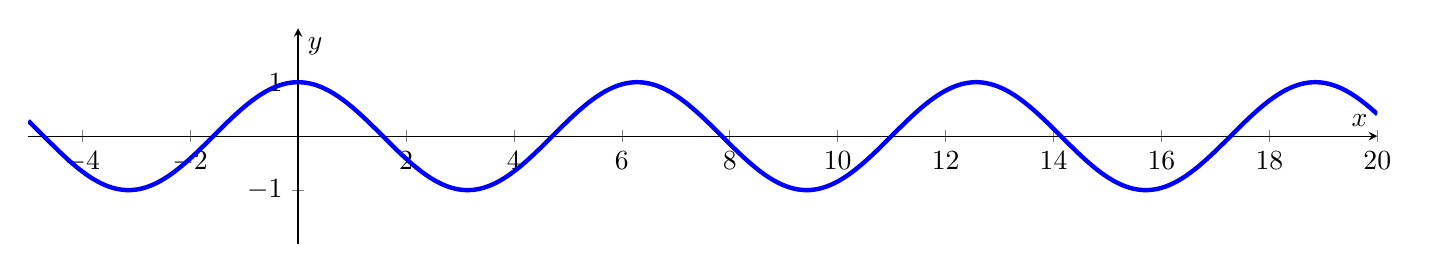
\begin{tikzpicture}
            \begin{axis}[
                    scale=2.5,
                    axis equal image,
                    samples=500,
                    axis lines=middle,
                    ymin=-2,ymax=2,
                    ytick={-1,1},
                    ylabel=$y$,
                    xlabel=$x$
                ]
                \addplot[domain=-5:20, black, ultra thick, color=blue]
                {cos(deg(x))};
            \end{axis}
        \end{tikzpicture}
    \end{image}
}

Remarks can simply be included in the running text, or by using
\verb|\begin{remark}|:

\begin{remark}[Properties of the absolute value (with $a$ a real number)]
    \begin{enumerate}
        \item Be careful: $|-a|= |a|$, but \textit{definitely
                  not} $\xcancel{|-a|=a}$

              $|-a|=a$ is \textsc{incorrect} if $a<0$. Indeed, if
              $a=-7$, then $|-a| = |-(-7)| {\color{red}\neq} -7 = a$
        \item $|a^2 + 1| = a^2 + 1$, because $a^2+1$ is always
              positive.
              % \item $|a^2 - 1| = ....$ \qquad(there is \textsc{no} simple general formula without $|\cdot|$)
    \end{enumerate}
\end{remark}

Examples use \verb|\begin{example}|.
By default, examples also provide the correct answer in the handout version,
while that is not the case for the exercises.

% \renewcommand{\choiceminimumverticalsize}{\vphantom{$\sqrt{2}$}} 

\begin{example}[Simple examples of absolute values]

    %\begin{xmmulticols}
    \begin{enumerate}
        \item $|5|=5$ and $|-5|=5$
        \item $|\sqrt{2}-1| =
              $\wordChoice{\choice[correct]{$\sqrt{2} -
                          1$}\choice{$1-\sqrt{2}$}}
        \item $|1-\sqrt{2}| =
              $\wordChoice{\choice[correct]{$\sqrt{2} -
                          1$}\choice{$1-\sqrt{2}$}}
        \item $|2-\sqrt{2}| = $\wordChoice{\choice{$\sqrt{2} -
                          2$}\choice[correct]{$2-\sqrt{2}$}}
    \end{enumerate}
    %\end{xmmulticols}
\end{example}

\end{document}